\documentclass[1p]{elsarticle_modified}
%\bibliographystyle{elsarticle-num}

%\usepackage[colorlinks]{hyperref}
%\usepackage{abbrmath_seonhwa} %\Abb, \Ascr, \Acal ,\Abf, \Afrak
\usepackage{amsfonts}
\usepackage{amssymb}
\usepackage{amsmath}
\usepackage{amsthm}
\usepackage{scalefnt}
\usepackage{amsbsy}
\usepackage{kotex}
\usepackage{caption}
\usepackage{subfig}
\usepackage{color}
\usepackage{graphicx}
\usepackage{xcolor} %% white, black, red, green, blue, cyan, magenta, yellow
\usepackage{float}
\usepackage{setspace}
\usepackage{hyperref}

\usepackage{tikz}
\usetikzlibrary{arrows}

\usepackage{multirow}
\usepackage{array} % fixed length table
\usepackage{hhline}

%%%%%%%%%%%%%%%%%%%%%
\makeatletter
\renewcommand*\env@matrix[1][\arraystretch]{%
	\edef\arraystretch{#1}%
	\hskip -\arraycolsep
	\let\@ifnextchar\new@ifnextchar
	\array{*\c@MaxMatrixCols c}}
\makeatother %https://tex.stackexchange.com/questions/14071/how-can-i-increase-the-line-spacing-in-a-matrix
%%%%%%%%%%%%%%%

\usepackage[normalem]{ulem}

\newcommand{\msout}[1]{\ifmmode\text{\sout{\ensuremath{#1}}}\else\sout{#1}\fi}
%SOURCE: \msout is \stkout macro in https://tex.stackexchange.com/questions/20609/strikeout-in-math-mode

\newcommand{\cancel}[1]{
	\ifmmode
	{\color{red}\msout{#1}}
	\else
	{\color{red}\sout{#1}}
	\fi
}

\newcommand{\add}[1]{
	{\color{blue}\uwave{#1}}
}

\newcommand{\replace}[2]{
	\ifmmode
	{\color{red}\msout{#1}}{\color{blue}\uwave{#2}}
	\else
	{\color{red}\sout{#1}}{\color{blue}\uwave{#2}}
	\fi
}

\newcommand{\Sol}{\mathcal{S}} %segment
\newcommand{\D}{D} %diagram
\newcommand{\A}{\mathcal{A}} %arc


%%%%%%%%%%%%%%%%%%%%%%%%%%%%%5 test

\def\sl{\operatorname{\textup{SL}}(2,\Cbb)}
\def\psl{\operatorname{\textup{PSL}}(2,\Cbb)}
\def\quan{\mkern 1mu \triangleright \mkern 1mu}

\theoremstyle{definition}
\newtheorem{thm}{Theorem}[section]
\newtheorem{prop}[thm]{Proposition}
\newtheorem{lem}[thm]{Lemma}
\newtheorem{ques}[thm]{Question}
\newtheorem{cor}[thm]{Corollary}
\newtheorem{defn}[thm]{Definition}
\newtheorem{exam}[thm]{Example}
\newtheorem{rmk}[thm]{Remark}
\newtheorem{alg}[thm]{Algorithm}

\newcommand{\I}{\sqrt{-1}}
\begin{document}

%\begin{frontmatter}
%
%\title{Boundary parabolic representations of knots up to 8 crossings}
%
%%% Group authors per affiliation:
%\author{Yunhi Cho} 
%\address{Department of Mathematics, University of Seoul, Seoul, Korea}
%\ead{yhcho@uos.ac.kr}
%
%
%\author{Seonhwa Kim} %\fnref{s_kim}}
%\address{Center for Geometry and Physics, Institute for Basic Science, Pohang, 37673, Korea}
%\ead{ryeona17@ibs.re.kr}
%
%\author{Hyuk Kim}
%\address{Department of Mathematical Sciences, Seoul National University, Seoul 08826, Korea}
%\ead{hyukkim@snu.ac.kr}
%
%\author{Seokbeom Yoon}
%\address{Department of Mathematical Sciences, Seoul National University, Seoul, 08826,  Korea}
%\ead{sbyoon15@snu.ac.kr}
%
%\begin{abstract}
%We find all boundary parabolic representation of knots up to 8 crossings.
%
%\end{abstract}
%\begin{keyword}
%    \MSC[2010] 57M25 
%\end{keyword}
%
%\end{frontmatter}

%\linenumbers
%\tableofcontents
%
\newcommand\colored[1]{\textcolor{white}{\rule[-0.35ex]{0.8em}{1.4ex}}\kern-0.8em\color{red} #1}%
%\newcommand\colored[1]{\textcolor{white}{ #1}\kern-2.17ex	\textcolor{white}{ #1}\kern-1.81ex	\textcolor{white}{ #1}\kern-2.15ex\color{red}#1	}

{\Large $\underline{12n_{0462}~(K12n_{0462})}$}

\setlength{\tabcolsep}{10pt}
\renewcommand{\arraystretch}{1.6}
\vspace{1cm}\begin{tabular}{m{100pt}>{\centering\arraybackslash}m{274pt}}
\multirow{5}{120pt}{
	\centering
	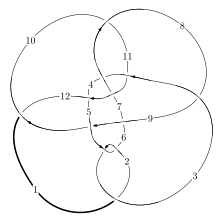
\includegraphics[width=112pt]{../../../GIT/diagram.site/Diagrams/png/2551_12n_0462.png}\\
\ \ \ A knot diagram\footnotemark}&
\allowdisplaybreaks
\textbf{Linearized knot diagam} \\
\cline{2-2}
 &
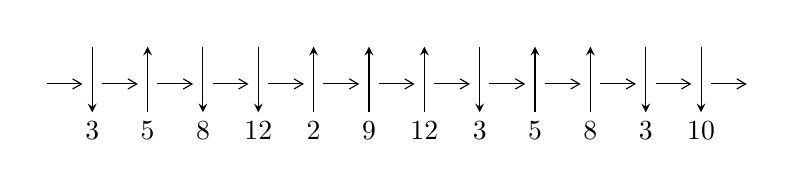
\begin{tikzpicture}[x=20pt, y=17pt]
	% nodes
	\node (C0) at (0, 0) {};
	\node (C1) at (1, 0) {};
	\node (C1U) at (1, +1) {};
	\node (C1D) at (1, -1) {3};

	\node (C2) at (2, 0) {};
	\node (C2U) at (2, +1) {};
	\node (C2D) at (2, -1) {5};

	\node (C3) at (3, 0) {};
	\node (C3U) at (3, +1) {};
	\node (C3D) at (3, -1) {8};

	\node (C4) at (4, 0) {};
	\node (C4U) at (4, +1) {};
	\node (C4D) at (4, -1) {12};

	\node (C5) at (5, 0) {};
	\node (C5U) at (5, +1) {};
	\node (C5D) at (5, -1) {2};

	\node (C6) at (6, 0) {};
	\node (C6U) at (6, +1) {};
	\node (C6D) at (6, -1) {9};

	\node (C7) at (7, 0) {};
	\node (C7U) at (7, +1) {};
	\node (C7D) at (7, -1) {12};

	\node (C8) at (8, 0) {};
	\node (C8U) at (8, +1) {};
	\node (C8D) at (8, -1) {3};

	\node (C9) at (9, 0) {};
	\node (C9U) at (9, +1) {};
	\node (C9D) at (9, -1) {5};

	\node (C10) at (10, 0) {};
	\node (C10U) at (10, +1) {};
	\node (C10D) at (10, -1) {8};

	\node (C11) at (11, 0) {};
	\node (C11U) at (11, +1) {};
	\node (C11D) at (11, -1) {3};

	\node (C12) at (12, 0) {};
	\node (C12U) at (12, +1) {};
	\node (C12D) at (12, -1) {10};
	\node (C13) at (13, 0) {};

	% arrows
	\draw[->,>={angle 60}]
	(C0) edge (C1) (C1) edge (C2) (C2) edge (C3) (C3) edge (C4) (C4) edge (C5) (C5) edge (C6) (C6) edge (C7) (C7) edge (C8) (C8) edge (C9) (C9) edge (C10) (C10) edge (C11) (C11) edge (C12) (C12) edge (C13) ;	\draw[->,>=stealth]
	(C1U) edge (C1D) (C2D) edge (C2U) (C3U) edge (C3D) (C4U) edge (C4D) (C5D) edge (C5U) (C6D) edge (C6U) (C7D) edge (C7U) (C8U) edge (C8D) (C9D) edge (C9U) (C10D) edge (C10U) (C11U) edge (C11D) (C12U) edge (C12D) ;
	\end{tikzpicture} \\
\hhline{~~} \\& 
\textbf{Solving Sequence} \\ \cline{2-2} 
 &
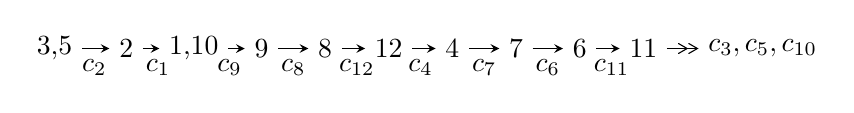
\begin{tikzpicture}[x=23pt, y=7pt]
	% node
	\node (A0) at (-1/8, 0) {3,5};
	\node (A1) at (1, 0) {2};
	\node (A2) at (33/16, 0) {1,10};
	\node (A3) at (25/8, 0) {9};
	\node (A4) at (33/8, 0) {8};
	\node (A5) at (41/8, 0) {12};
	\node (A6) at (49/8, 0) {4};
	\node (A7) at (57/8, 0) {7};
	\node (A8) at (65/8, 0) {6};
	\node (A9) at (73/8, 0) {11};
	\node (C1) at (1/2, -1) {$c_{2}$};
	\node (C2) at (3/2, -1) {$c_{1}$};
	\node (C3) at (21/8, -1) {$c_{9}$};
	\node (C4) at (29/8, -1) {$c_{8}$};
	\node (C5) at (37/8, -1) {$c_{12}$};
	\node (C6) at (45/8, -1) {$c_{4}$};
	\node (C7) at (53/8, -1) {$c_{7}$};
	\node (C8) at (61/8, -1) {$c_{6}$};
	\node (C9) at (69/8, -1) {$c_{11}$};
	\node (A10) at (11, 0) {$c_{3},c_{5},c_{10}$};

	% edge
	\draw[->,>=stealth]	
	(A0) edge (A1) (A1) edge (A2) (A2) edge (A3) (A3) edge (A4) (A4) edge (A5) (A5) edge (A6) (A6) edge (A7) (A7) edge (A8) (A8) edge (A9) ;
	\draw[->>,>={angle 60}]	
	(A9) edge (A10);
\end{tikzpicture} \\ 

\end{tabular} \\

\footnotetext{
The image of knot diagram is generated by the software ``\textbf{Draw programme}" developed by Andrew Bartholomew(\url{http://www.layer8.co.uk/maths/draw/index.htm\#Running-draw}), where we modified some parts for our purpose(\url{https://github.com/CATsTAILs/LinksPainter}).
}\phantom \\ \newline 
\centering \textbf{Ideals for irreducible components\footnotemark of $X_{\text{par}}$} 
 
\begin{align*}
I^u_{1}&=\langle 
-149788246 u^{19}+735301154 u^{18}+\cdots+16882806339 b-24202510048,\\
\phantom{I^u_{1}}&\phantom{= \langle  }-38489542585 u^{19}+46865050127 u^{18}+\cdots+16882806339 a-207132124495,\\
\phantom{I^u_{1}}&\phantom{= \langle  }u^{20}- u^{19}+\cdots+11 u+1\rangle \\
I^u_{2}&=\langle 
u^2+b+1,\;u^5-2 u^4+5 u^3-6 u^2+3 a+6 u-1,\;u^6- u^5+5 u^4-4 u^3+7 u^2-2 u+3\rangle \\
I^u_{3}&=\langle 
b- u,\;a- u,\;u^2+u+1\rangle \\
\\
\end{align*}
\raggedright * 3 irreducible components of $\dim_{\mathbb{C}}=0$, with total 28 representations.\\
\footnotetext{All coefficients of polynomials are rational numbers. But the coefficients are sometimes approximated in decimal forms when there is not enough margin.}
\newpage
\renewcommand{\arraystretch}{1}
\centering \section*{I. $I^u_{1}= \langle -1.50\times10^{8} u^{19}+7.35\times10^{8} u^{18}+\cdots+1.69\times10^{10} b-2.42\times10^{10},\;-3.85\times10^{10} u^{19}+4.69\times10^{10} u^{18}+\cdots+1.69\times10^{10} a-2.07\times10^{11},\;u^{20}- u^{19}+\cdots+11 u+1 \rangle$}
\flushleft \textbf{(i) Arc colorings}\\
\begin{tabular}{m{7pt} m{180pt} m{7pt} m{180pt} }
\flushright $a_{3}=$&$\begin{pmatrix}1\\0\end{pmatrix}$ \\
\flushright $a_{5}=$&$\begin{pmatrix}0\\u\end{pmatrix}$ \\
\flushright $a_{2}=$&$\begin{pmatrix}1\\u^2\end{pmatrix}$ \\
\flushright $a_{1}=$&$\begin{pmatrix}u^2+1\\u^2\end{pmatrix}$ \\
\flushright $a_{10}=$&$\begin{pmatrix}2.27981 u^{19}-2.77590 u^{18}+\cdots+74.2433 u+12.2688\\0.00887224 u^{19}-0.0435533 u^{18}+\cdots+9.24808 u+1.43356\end{pmatrix}$ \\
\flushright $a_{9}=$&$\begin{pmatrix}2.27981 u^{19}-2.77590 u^{18}+\cdots+74.2433 u+12.2688\\0.0852452 u^{19}-0.0369754 u^{18}+\cdots+12.4253 u+1.92966\end{pmatrix}$ \\
\flushright $a_{8}=$&$\begin{pmatrix}2.36505 u^{19}-2.81288 u^{18}+\cdots+86.6686 u+14.1985\\0.0852452 u^{19}-0.0369754 u^{18}+\cdots+12.4253 u+1.92966\end{pmatrix}$ \\
\flushright $a_{12}=$&$\begin{pmatrix}-0.00359098 u^{19}+0.391699 u^{18}+\cdots+9.11164 u+4.91265\\0.327637 u^{19}-0.499312 u^{18}+\cdots+0.549227 u+0.495867\end{pmatrix}$ \\
\flushright $a_{4}=$&$\begin{pmatrix}0.627286 u^{19}-0.803555 u^{18}+\cdots+31.8391 u+2.03483\\0.253178 u^{19}-0.0827151 u^{18}+\cdots+12.4507 u+0.748328\end{pmatrix}$ \\
\flushright $a_{7}=$&$\begin{pmatrix}1.92966 u^{19}-2.01490 u^{18}+\cdots+73.2986 u+8.80089\\0.509356 u^{19}-0.765818 u^{18}+\cdots+2.50917 u+0.308552\end{pmatrix}$ \\
\flushright $a_{6}=$&$\begin{pmatrix}- u\\- u^3- u\end{pmatrix}$ \\
\flushright $a_{11}=$&$\begin{pmatrix}0.324046 u^{19}-0.107613 u^{18}+\cdots+9.66087 u+5.40852\\0.327637 u^{19}-0.499312 u^{18}+\cdots+0.549227 u+0.495867\end{pmatrix}$\\&\end{tabular}
\flushleft \textbf{(ii) Obstruction class $= -1$}\\~\\
\flushleft \textbf{(iii) Cusp Shapes $= -\frac{12674828861}{16882806339} u^{19}+\frac{1750449202}{2411829477} u^{18}+\cdots-\frac{510127682849}{16882806339} u+\frac{10680247402}{16882806339}$}\\~\\
\newpage\renewcommand{\arraystretch}{1}
\flushleft \textbf{(iv) u-Polynomials at the component}\newline \\
\begin{tabular}{m{50pt}|m{274pt}}
Crossings & \hspace{64pt}u-Polynomials at each crossing \\
\hline $$\begin{aligned}c_{1}\end{aligned}$$&$\begin{aligned}
&u^{20}+27 u^{19}+\cdots-27 u+1
\end{aligned}$\\
\hline $$\begin{aligned}c_{2},c_{5}\end{aligned}$$&$\begin{aligned}
&u^{20}+u^{19}+\cdots-11 u+1
\end{aligned}$\\
\hline $$\begin{aligned}c_{3},c_{8}\end{aligned}$$&$\begin{aligned}
&u^{20}- u^{19}+\cdots+11 u+1
\end{aligned}$\\
\hline $$\begin{aligned}c_{4}\end{aligned}$$&$\begin{aligned}
&u^{20}+2 u^{19}+\cdots-27 u+51
\end{aligned}$\\
\hline $$\begin{aligned}c_{6}\end{aligned}$$&$\begin{aligned}
&u^{20}+16 u^{18}+\cdots-16 u+52
\end{aligned}$\\
\hline $$\begin{aligned}c_{7}\end{aligned}$$&$\begin{aligned}
&u^{20}-3 u^{19}+\cdots+109 u^2+21
\end{aligned}$\\
\hline $$\begin{aligned}c_{9}\end{aligned}$$&$\begin{aligned}
&u^{20}-2 u^{19}+\cdots+27 u+51
\end{aligned}$\\
\hline $$\begin{aligned}c_{10}\end{aligned}$$&$\begin{aligned}
&u^{20}+5 u^{19}+\cdots+57 u+7
\end{aligned}$\\
\hline $$\begin{aligned}c_{11}\end{aligned}$$&$\begin{aligned}
&u^{20}+16 u^{18}+\cdots+16 u+52
\end{aligned}$\\
\hline $$\begin{aligned}c_{12}\end{aligned}$$&$\begin{aligned}
&u^{20}-5 u^{19}+\cdots-57 u+7
\end{aligned}$\\
\hline
\end{tabular}\\~\\
\newpage\renewcommand{\arraystretch}{1}
\flushleft \textbf{(v) Riley Polynomials at the component}\newline \\
\begin{tabular}{m{50pt}|m{274pt}}
Crossings & \hspace{64pt}Riley Polynomials at each crossing \\
\hline $$\begin{aligned}c_{1}\end{aligned}$$&$\begin{aligned}
&y^{20}-61 y^{19}+\cdots+169 y+1
\end{aligned}$\\
\hline $$\begin{aligned}c_{2},c_{3},c_{5}\\c_{8}\end{aligned}$$&$\begin{aligned}
&y^{20}+27 y^{19}+\cdots-27 y+1
\end{aligned}$\\
\hline $$\begin{aligned}c_{4},c_{9}\end{aligned}$$&$\begin{aligned}
&y^{20}+18 y^{19}+\cdots+17835 y+2601
\end{aligned}$\\
\hline $$\begin{aligned}c_{6},c_{11}\end{aligned}$$&$\begin{aligned}
&y^{20}+32 y^{19}+\cdots+7024 y+2704
\end{aligned}$\\
\hline $$\begin{aligned}c_{7}\end{aligned}$$&$\begin{aligned}
&y^{20}-33 y^{19}+\cdots+4578 y+441
\end{aligned}$\\
\hline $$\begin{aligned}c_{10},c_{12}\end{aligned}$$&$\begin{aligned}
&y^{20}-15 y^{19}+\cdots-1835 y+49
\end{aligned}$\\
\hline
\end{tabular}\\~\\
\newpage\flushleft \textbf{(vi) Complex Volumes and Cusp Shapes}
$$\begin{array}{c|c|c}  
\text{Solutions to }I^u_{1}& \I (\text{vol} + \sqrt{-1}CS) & \text{Cusp shape}\\
 \hline 
\begin{aligned}
u &= \phantom{-}0.160143 + 0.768509 I \\
a &= -0.394995 - 1.004840 I \\
b &= -0.636041 - 0.396936 I\end{aligned}
 & -1.10947 - 1.48655 I & -5.12329 + 2.41841 I \\ \hline\begin{aligned}
u &= \phantom{-}0.160143 - 0.768509 I \\
a &= -0.394995 + 1.004840 I \\
b &= -0.636041 + 0.396936 I\end{aligned}
 & -1.10947 + 1.48655 I & -5.12329 - 2.41841 I \\ \hline\begin{aligned}
u &= -0.484926 + 0.607075 I \\
a &= \phantom{-}0.577525 - 0.647733 I \\
b &= -0.026523 - 0.353444 I\end{aligned}
 & \phantom{-0.000000 } -1.43025 I & \phantom{-0.000000 -}0. + 5.92138 I \\ \hline\begin{aligned}
u &= -0.484926 - 0.607075 I \\
a &= \phantom{-}0.577525 + 0.647733 I \\
b &= -0.026523 + 0.353444 I\end{aligned}
 & \phantom{-0.000000 -}1.43025 I & \phantom{-0.000000 } 0. - 5.92138 I \\ \hline\begin{aligned}
u &= -0.08307 + 1.42113 I \\
a &= -0.271547 + 1.012220 I \\
b &= -1.110600 + 0.490957 I\end{aligned}
 & \phantom{-}3.72589 - 1.03786 I & \phantom{-}1.73919 + 0.58908 I \\ \hline\begin{aligned}
u &= -0.08307 - 1.42113 I \\
a &= -0.271547 - 1.012220 I \\
b &= -1.110600 - 0.490957 I\end{aligned}
 & \phantom{-}3.72589 + 1.03786 I & \phantom{-}1.73919 - 0.58908 I \\ \hline\begin{aligned}
u &= \phantom{-}1.18575 + 0.83320 I \\
a &= \phantom{-}0.626136 + 0.573895 I \\
b &= \phantom{-}0.569199 + 0.092819 I\end{aligned}
 & \phantom{-}8.81653 + 3.95168 I & \phantom{-}0.25331 - 3.24699 I \\ \hline\begin{aligned}
u &= \phantom{-}1.18575 - 0.83320 I \\
a &= \phantom{-}0.626136 - 0.573895 I \\
b &= \phantom{-}0.569199 - 0.092819 I\end{aligned}
 & \phantom{-}8.81653 - 3.95168 I & \phantom{-}0.25331 + 3.24699 I \\ \hline\begin{aligned}
u &= -0.104414 + 0.507262 I \\
a &= \phantom{-}1.44705 - 1.63599 I \\
b &= \phantom{-}0.64554 + 1.51309 I\end{aligned}
 & \phantom{-}10.23410 - 0.33723 I & \phantom{-}1.46943 - 0.53181 I \\ \hline\begin{aligned}
u &= -0.104414 - 0.507262 I \\
a &= \phantom{-}1.44705 + 1.63599 I \\
b &= \phantom{-}0.64554 - 1.51309 I\end{aligned}
 & \phantom{-}10.23410 + 0.33723 I & \phantom{-}1.46943 + 0.53181 I\\
 \hline 
 \end{array}$$\newpage$$\begin{array}{c|c|c}  
\text{Solutions to }I^u_{1}& \I (\text{vol} + \sqrt{-1}CS) & \text{Cusp shape}\\
 \hline 
\begin{aligned}
u &= -0.32507 + 1.48224 I \\
a &= \phantom{-}0.843038 - 0.018166 I \\
b &= \phantom{-}1.69755 - 0.64672 I\end{aligned}
 & -3.72589 - 1.03786 I & -1.73919 + 0.58908 I \\ \hline\begin{aligned}
u &= -0.32507 - 1.48224 I \\
a &= \phantom{-}0.843038 + 0.018166 I \\
b &= \phantom{-}1.69755 + 0.64672 I\end{aligned}
 & -3.72589 + 1.03786 I & -1.73919 - 0.58908 I \\ \hline\begin{aligned}
u &= -0.11912 + 1.73852 I \\
a &= -1.211980 - 0.171698 I \\
b &= -2.38905 - 0.18528 I\end{aligned}
 & -8.81653 - 3.95168 I & -0.25331 + 3.24699 I \\ \hline\begin{aligned}
u &= -0.11912 - 1.73852 I \\
a &= -1.211980 + 0.171698 I \\
b &= -2.38905 + 0.18528 I\end{aligned}
 & -8.81653 + 3.95168 I & -0.25331 - 3.24699 I \\ \hline\begin{aligned}
u &= \phantom{-}0.11567 + 1.76293 I \\
a &= \phantom{-}0.697284 + 0.000472 I \\
b &= \phantom{-}2.05356 + 0.22436 I\end{aligned}
 & -10.23410 + 0.33723 I & -1.46943 + 0.53181 I \\ \hline\begin{aligned}
u &= \phantom{-}0.11567 - 1.76293 I \\
a &= \phantom{-}0.697284 - 0.000472 I \\
b &= \phantom{-}2.05356 - 0.22436 I\end{aligned}
 & -10.23410 - 0.33723 I & -1.46943 - 0.53181 I \\ \hline\begin{aligned}
u &= \phantom{-}0.32058 + 1.78463 I \\
a &= -0.974674 + 0.336167 I \\
b &= -2.29883 + 0.36675 I\end{aligned}
 & \phantom{-0.000000 -}9.75717 I & \phantom{-0.000000 } 0. - 4.10936 I \\ \hline\begin{aligned}
u &= \phantom{-}0.32058 - 1.78463 I \\
a &= -0.974674 - 0.336167 I \\
b &= -2.29883 - 0.36675 I\end{aligned}
 & \phantom{-0.000000 } -9.75717 I & \phantom{-0.000000 -}0. + 4.10936 I \\ \hline\begin{aligned}
u &= -0.165551 + 0.073534 I \\
a &= \phantom{-}2.16216 + 4.82053 I \\
b &= -0.004791 + 0.715102 I\end{aligned}
 & \phantom{-}1.10947 + 1.48655 I & \phantom{-}5.12329 - 2.41841 I \\ \hline\begin{aligned}
u &= -0.165551 - 0.073534 I \\
a &= \phantom{-}2.16216 - 4.82053 I \\
b &= -0.004791 - 0.715102 I\end{aligned}
 & \phantom{-}1.10947 - 1.48655 I & \phantom{-}5.12329 + 2.41841 I\\
 \hline 
 \end{array}$$\newpage\newpage\renewcommand{\arraystretch}{1}
\centering \section*{II. $I^u_{2}= \langle u^2+b+1,\;u^5-2 u^4+5 u^3-6 u^2+3 a+6 u-1,\;u^6- u^5+5 u^4-4 u^3+7 u^2-2 u+3 \rangle$}
\flushleft \textbf{(i) Arc colorings}\\
\begin{tabular}{m{7pt} m{180pt} m{7pt} m{180pt} }
\flushright $a_{3}=$&$\begin{pmatrix}1\\0\end{pmatrix}$ \\
\flushright $a_{5}=$&$\begin{pmatrix}0\\u\end{pmatrix}$ \\
\flushright $a_{2}=$&$\begin{pmatrix}1\\u^2\end{pmatrix}$ \\
\flushright $a_{1}=$&$\begin{pmatrix}u^2+1\\u^2\end{pmatrix}$ \\
\flushright $a_{10}=$&$\begin{pmatrix}-\frac{1}{3} u^5+\frac{2}{3} u^4+\cdots-2 u+\frac{1}{3}\\- u^2-1\end{pmatrix}$ \\
\flushright $a_{9}=$&$\begin{pmatrix}-\frac{1}{3} u^5+\frac{2}{3} u^4+\cdots-2 u+\frac{1}{3}\\\frac{1}{3} u^5- u^4+\cdots+\frac{5}{3} u-2\end{pmatrix}$ \\
\flushright $a_{8}=$&$\begin{pmatrix}-\frac{1}{3} u^4-\frac{5}{3} u^2-\frac{1}{3} u-\frac{5}{3}\\\frac{1}{3} u^5- u^4+\cdots+\frac{5}{3} u-2\end{pmatrix}$ \\
\flushright $a_{12}=$&$\begin{pmatrix}-\frac{1}{3} u^5+\frac{2}{3} u^4+\cdots-2 u+\frac{7}{3}\\-\frac{2}{3} u^5+u^4+\cdots-\frac{4}{3} u+1\end{pmatrix}$ \\
\flushright $a_{4}=$&$\begin{pmatrix}\frac{2}{3} u^5+\frac{1}{3} u^4+\cdots+\frac{2}{3} u+\frac{5}{3}\\\frac{2}{3} u^5+\frac{7}{3} u^3-\frac{1}{3} u^2+\frac{4}{3} u-1\end{pmatrix}$ \\
\flushright $a_{7}=$&$\begin{pmatrix}-\frac{2}{3} u^5+\frac{1}{3} u^4+\cdots- u-\frac{1}{3}\\u^3+u^2+2 u+1\end{pmatrix}$ \\
\flushright $a_{6}=$&$\begin{pmatrix}u\\u^3+u\end{pmatrix}$ \\
\flushright $a_{11}=$&$\begin{pmatrix}- u^5+\frac{5}{3} u^4+\cdots-\frac{10}{3} u+\frac{10}{3}\\-\frac{2}{3} u^5+u^4+\cdots-\frac{4}{3} u+1\end{pmatrix}$\\&\end{tabular}
\flushleft \textbf{(ii) Obstruction class $= 1$}\\~\\
\flushleft \textbf{(iii) Cusp Shapes $= u^5-3 u^4+5 u^3-11 u^2+8 u-6$}\\~\\
\newpage\renewcommand{\arraystretch}{1}
\flushleft \textbf{(iv) u-Polynomials at the component}\newline \\
\begin{tabular}{m{50pt}|m{274pt}}
Crossings & \hspace{64pt}u-Polynomials at each crossing \\
\hline $$\begin{aligned}c_{1}\end{aligned}$$&$\begin{aligned}
&u^6-9 u^5+31 u^4-56 u^3+63 u^2-38 u+9
\end{aligned}$\\
\hline $$\begin{aligned}c_{2},c_{8}\end{aligned}$$&$\begin{aligned}
&u^6- u^5+5 u^4-4 u^3+7 u^2-2 u+3
\end{aligned}$\\
\hline $$\begin{aligned}c_{3},c_{5}\end{aligned}$$&$\begin{aligned}
&u^6+u^5+5 u^4+4 u^3+7 u^2+2 u+3
\end{aligned}$\\
\hline $$\begin{aligned}c_{4}\end{aligned}$$&$\begin{aligned}
&u^6+2 u^4+3 u^3+2 u^2+1
\end{aligned}$\\
\hline $$\begin{aligned}c_{6}\end{aligned}$$&$\begin{aligned}
&u^6- u^5+4 u^4-2 u^3-8 u^2+6 u+9
\end{aligned}$\\
\hline $$\begin{aligned}c_{7}\end{aligned}$$&$\begin{aligned}
&u^6-3 u^5+u^4-2 u^3+6 u^2+5 u+1
\end{aligned}$\\
\hline $$\begin{aligned}c_{9}\end{aligned}$$&$\begin{aligned}
&u^6+2 u^4-3 u^3+2 u^2+1
\end{aligned}$\\
\hline $$\begin{aligned}c_{10}\end{aligned}$$&$\begin{aligned}
&u^6-3 u^5+5 u^3- u^2-2 u+3
\end{aligned}$\\
\hline $$\begin{aligned}c_{11}\end{aligned}$$&$\begin{aligned}
&u^6+u^5+4 u^4+2 u^3-8 u^2-6 u+9
\end{aligned}$\\
\hline $$\begin{aligned}c_{12}\end{aligned}$$&$\begin{aligned}
&u^6+3 u^5-5 u^3- u^2+2 u+3
\end{aligned}$\\
\hline
\end{tabular}\\~\\
\newpage\renewcommand{\arraystretch}{1}
\flushleft \textbf{(v) Riley Polynomials at the component}\newline \\
\begin{tabular}{m{50pt}|m{274pt}}
Crossings & \hspace{64pt}Riley Polynomials at each crossing \\
\hline $$\begin{aligned}c_{1}\end{aligned}$$&$\begin{aligned}
&y^6-19 y^5+79 y^4+104 y^3+271 y^2-310 y+81
\end{aligned}$\\
\hline $$\begin{aligned}c_{2},c_{3},c_{5}\\c_{8}\end{aligned}$$&$\begin{aligned}
&y^6+9 y^5+31 y^4+56 y^3+63 y^2+38 y+9
\end{aligned}$\\
\hline $$\begin{aligned}c_{4},c_{9}\end{aligned}$$&$\begin{aligned}
&y^6+4 y^5+8 y^4+y^3+8 y^2+4 y+1
\end{aligned}$\\
\hline $$\begin{aligned}c_{6},c_{11}\end{aligned}$$&$\begin{aligned}
&y^6+7 y^5-4 y^4-38 y^3+160 y^2-180 y+81
\end{aligned}$\\
\hline $$\begin{aligned}c_{7}\end{aligned}$$&$\begin{aligned}
&y^6-7 y^5+y^4+40 y^3+58 y^2-13 y+1
\end{aligned}$\\
\hline $$\begin{aligned}c_{10},c_{12}\end{aligned}$$&$\begin{aligned}
&y^6-9 y^5+28 y^4-31 y^3+21 y^2-10 y+9
\end{aligned}$\\
\hline
\end{tabular}\\~\\
\newpage\flushleft \textbf{(vi) Complex Volumes and Cusp Shapes}
$$\begin{array}{c|c|c}  
\text{Solutions to }I^u_{2}& \I (\text{vol} + \sqrt{-1}CS) & \text{Cusp shape}\\
 \hline 
\begin{aligned}
u &= \phantom{-}0.615293 + 1.007340 I \\
a &= -0.488052 - 0.086507 I \\
b &= -0.363854 - 1.239620 I\end{aligned}
 & \phantom{-}10.45590 + 2.33911 I & \phantom{-}2.00744 - 2.34673 I \\ \hline\begin{aligned}
u &= \phantom{-}0.615293 - 1.007340 I \\
a &= -0.488052 + 0.086507 I \\
b &= -0.363854 + 1.239620 I\end{aligned}
 & \phantom{-}10.45590 - 2.33911 I & \phantom{-}2.00744 + 2.34673 I \\ \hline\begin{aligned}
u &= -0.061440 + 0.817267 I \\
a &= -0.744380 - 0.966777 I \\
b &= -0.335850 + 0.100426 I\end{aligned}
 & \phantom{-0.000000 } -2.22275 I & \phantom{-0.000000 -}0. + 4.90360 I \\ \hline\begin{aligned}
u &= -0.061440 - 0.817267 I \\
a &= -0.744380 + 0.966777 I \\
b &= -0.335850 - 0.100426 I\end{aligned}
 & \phantom{-0.000000 -}2.22275 I & \phantom{-0.000000 } 0. - 4.90360 I \\ \hline\begin{aligned}
u &= -0.05385 + 1.78958 I \\
a &= \phantom{-}0.899099 + 0.320901 I \\
b &= \phantom{-}2.19970 + 0.19275 I\end{aligned}
 & -10.45590 - 2.33911 I & -2.00744 + 2.34673 I \\ \hline\begin{aligned}
u &= -0.05385 - 1.78958 I \\
a &= \phantom{-}0.899099 - 0.320901 I \\
b &= \phantom{-}2.19970 - 0.19275 I\end{aligned}
 & -10.45590 + 2.33911 I & -2.00744 - 2.34673 I\\
 \hline 
 \end{array}$$\newpage\newpage\renewcommand{\arraystretch}{1}
\centering \section*{III. $I^u_{3}= \langle b- u,\;a- u,\;u^2+u+1 \rangle$}
\flushleft \textbf{(i) Arc colorings}\\
\begin{tabular}{m{7pt} m{180pt} m{7pt} m{180pt} }
\flushright $a_{3}=$&$\begin{pmatrix}1\\0\end{pmatrix}$ \\
\flushright $a_{5}=$&$\begin{pmatrix}0\\u\end{pmatrix}$ \\
\flushright $a_{2}=$&$\begin{pmatrix}1\\- u-1\end{pmatrix}$ \\
\flushright $a_{1}=$&$\begin{pmatrix}- u\\- u-1\end{pmatrix}$ \\
\flushright $a_{10}=$&$\begin{pmatrix}u\\u\end{pmatrix}$ \\
\flushright $a_{9}=$&$\begin{pmatrix}u\\u+1\end{pmatrix}$ \\
\flushright $a_{8}=$&$\begin{pmatrix}2 u+1\\u+1\end{pmatrix}$ \\
\flushright $a_{12}=$&$\begin{pmatrix}1\\0\end{pmatrix}$ \\
\flushright $a_{4}=$&$\begin{pmatrix}u\\u\end{pmatrix}$ \\
\flushright $a_{7}=$&$\begin{pmatrix}u\\u+1\end{pmatrix}$ \\
\flushright $a_{6}=$&$\begin{pmatrix}u\\u+1\end{pmatrix}$ \\
\flushright $a_{11}=$&$\begin{pmatrix}1\\0\end{pmatrix}$\\&\end{tabular}
\flushleft \textbf{(ii) Obstruction class $= 1$}\\~\\
\flushleft \textbf{(iii) Cusp Shapes $= 0$}\\~\\
\newpage\renewcommand{\arraystretch}{1}
\flushleft \textbf{(iv) u-Polynomials at the component}\newline \\
\begin{tabular}{m{50pt}|m{274pt}}
Crossings & \hspace{64pt}u-Polynomials at each crossing \\
\hline $$\begin{aligned}c_{1},c_{3},c_{4}\\c_{5},c_{10}\end{aligned}$$&$\begin{aligned}
&u^2- u+1
\end{aligned}$\\
\hline $$\begin{aligned}c_{2},c_{7},c_{8}\\c_{9},c_{12}\end{aligned}$$&$\begin{aligned}
&u^2+u+1
\end{aligned}$\\
\hline $$\begin{aligned}c_{6},c_{11}\end{aligned}$$&$\begin{aligned}
&u^2
\end{aligned}$\\
\hline
\end{tabular}\\~\\
\newpage\renewcommand{\arraystretch}{1}
\flushleft \textbf{(v) Riley Polynomials at the component}\newline \\
\begin{tabular}{m{50pt}|m{274pt}}
Crossings & \hspace{64pt}Riley Polynomials at each crossing \\
\hline $$\begin{aligned}c_{1},c_{2},c_{3}\\c_{4},c_{5},c_{7}\\c_{8},c_{9},c_{10}\\c_{12}\end{aligned}$$&$\begin{aligned}
&y^2+y+1
\end{aligned}$\\
\hline $$\begin{aligned}c_{6},c_{11}\end{aligned}$$&$\begin{aligned}
&y^2
\end{aligned}$\\
\hline
\end{tabular}\\~\\
\newpage\flushleft \textbf{(vi) Complex Volumes and Cusp Shapes}
$$\begin{array}{c|c|c}  
\text{Solutions to }I^u_{3}& \I (\text{vol} + \sqrt{-1}CS) & \text{Cusp shape}\\
 \hline 
\begin{aligned}
u &= -0.500000 + 0.866025 I \\
a &= -0.500000 + 0.866025 I \\
b &= -0.500000 + 0.866025 I\end{aligned}
 & \phantom{-0.000000 } 0 & \phantom{-0.000000 } 0 \\ \hline\begin{aligned}
u &= -0.500000 - 0.866025 I \\
a &= -0.500000 - 0.866025 I \\
b &= -0.500000 - 0.866025 I\end{aligned}
 & \phantom{-0.000000 } 0 & \phantom{-0.000000 } 0\\
 \hline 
 \end{array}$$\newpage
\newpage\renewcommand{\arraystretch}{1}
\centering \section*{ IV. u-Polynomials}
\begin{tabular}{m{50pt}|m{274pt}}
Crossings & \hspace{64pt}u-Polynomials at each crossing \\
\hline $$\begin{aligned}c_{1}\end{aligned}$$&$\begin{aligned}
&(u^2- u+1)(u^6-9 u^5+31 u^4-56 u^3+63 u^2-38 u+9)\\
&\cdot(u^{20}+27 u^{19}+\cdots-27 u+1)
\end{aligned}$\\
\hline $$\begin{aligned}c_{2}\end{aligned}$$&$\begin{aligned}
&(u^2+u+1)(u^6- u^5+5 u^4-4 u^3+7 u^2-2 u+3)\\
&\cdot(u^{20}+u^{19}+\cdots-11 u+1)
\end{aligned}$\\
\hline $$\begin{aligned}c_{3}\end{aligned}$$&$\begin{aligned}
&(u^2- u+1)(u^6+u^5+5 u^4+4 u^3+7 u^2+2 u+3)\\
&\cdot(u^{20}- u^{19}+\cdots+11 u+1)
\end{aligned}$\\
\hline $$\begin{aligned}c_{4}\end{aligned}$$&$\begin{aligned}
&(u^2- u+1)(u^6+2 u^4+\cdots+2 u^2+1)(u^{20}+2 u^{19}+\cdots-27 u+51)
\end{aligned}$\\
\hline $$\begin{aligned}c_{5}\end{aligned}$$&$\begin{aligned}
&(u^2- u+1)(u^6+u^5+5 u^4+4 u^3+7 u^2+2 u+3)\\
&\cdot(u^{20}+u^{19}+\cdots-11 u+1)
\end{aligned}$\\
\hline $$\begin{aligned}c_{6}\end{aligned}$$&$\begin{aligned}
&u^2(u^6- u^5+\cdots+6 u+9)(u^{20}+16 u^{18}+\cdots-16 u+52)
\end{aligned}$\\
\hline $$\begin{aligned}c_{7}\end{aligned}$$&$\begin{aligned}
&(u^2+u+1)(u^6-3 u^5+u^4-2 u^3+6 u^2+5 u+1)\\
&\cdot(u^{20}-3 u^{19}+\cdots+109 u^2+21)
\end{aligned}$\\
\hline $$\begin{aligned}c_{8}\end{aligned}$$&$\begin{aligned}
&(u^2+u+1)(u^6- u^5+5 u^4-4 u^3+7 u^2-2 u+3)\\
&\cdot(u^{20}- u^{19}+\cdots+11 u+1)
\end{aligned}$\\
\hline $$\begin{aligned}c_{9}\end{aligned}$$&$\begin{aligned}
&(u^2+u+1)(u^6+2 u^4+\cdots+2 u^2+1)(u^{20}-2 u^{19}+\cdots+27 u+51)
\end{aligned}$\\
\hline $$\begin{aligned}c_{10}\end{aligned}$$&$\begin{aligned}
&(u^2- u+1)(u^6-3 u^5+\cdots-2 u+3)(u^{20}+5 u^{19}+\cdots+57 u+7)
\end{aligned}$\\
\hline $$\begin{aligned}c_{11}\end{aligned}$$&$\begin{aligned}
&u^2(u^6+u^5+\cdots-6 u+9)(u^{20}+16 u^{18}+\cdots+16 u+52)
\end{aligned}$\\
\hline $$\begin{aligned}c_{12}\end{aligned}$$&$\begin{aligned}
&(u^2+u+1)(u^6+3 u^5+\cdots+2 u+3)(u^{20}-5 u^{19}+\cdots-57 u+7)
\end{aligned}$\\
\hline
\end{tabular}\newpage\renewcommand{\arraystretch}{1}
\centering \section*{ V. Riley Polynomials}
\begin{tabular}{m{50pt}|m{274pt}}
Crossings & \hspace{64pt}Riley Polynomials at each crossing \\
\hline $$\begin{aligned}c_{1}\end{aligned}$$&$\begin{aligned}
&(y^2+y+1)(y^6-19 y^5+79 y^4+104 y^3+271 y^2-310 y+81)\\
&\cdot(y^{20}-61 y^{19}+\cdots+169 y+1)
\end{aligned}$\\
\hline $$\begin{aligned}c_{2},c_{3},c_{5}\\c_{8}\end{aligned}$$&$\begin{aligned}
&(y^2+y+1)(y^6+9 y^5+31 y^4+56 y^3+63 y^2+38 y+9)\\
&\cdot(y^{20}+27 y^{19}+\cdots-27 y+1)
\end{aligned}$\\
\hline $$\begin{aligned}c_{4},c_{9}\end{aligned}$$&$\begin{aligned}
&(y^2+y+1)(y^6+4 y^5+8 y^4+y^3+8 y^2+4 y+1)\\
&\cdot(y^{20}+18 y^{19}+\cdots+17835 y+2601)
\end{aligned}$\\
\hline $$\begin{aligned}c_{6},c_{11}\end{aligned}$$&$\begin{aligned}
&y^2(y^6+7 y^5-4 y^4-38 y^3+160 y^2-180 y+81)\\
&\cdot(y^{20}+32 y^{19}+\cdots+7024 y+2704)
\end{aligned}$\\
\hline $$\begin{aligned}c_{7}\end{aligned}$$&$\begin{aligned}
&(y^2+y+1)(y^6-7 y^5+y^4+40 y^3+58 y^2-13 y+1)\\
&\cdot(y^{20}-33 y^{19}+\cdots+4578 y+441)
\end{aligned}$\\
\hline $$\begin{aligned}c_{10},c_{12}\end{aligned}$$&$\begin{aligned}
&(y^2+y+1)(y^6-9 y^5+28 y^4-31 y^3+21 y^2-10 y+9)\\
&\cdot(y^{20}-15 y^{19}+\cdots-1835 y+49)
\end{aligned}$\\
\hline
\end{tabular}
\vskip 2pc
\end{document}